\documentclass[tikz, 12pt]{standalone}

\usepackage{xcolor}
\definecolor{colora}{RGB}{214,76,71}
\definecolor{colorg}{RGB}{84,175,216}
\definecolor{colort}{RGB}{98,174,17}
\definecolor{colorc}{RGB}{253,205,103}
\definecolor{colorn}{RGB}{ 45,45,45}
\definecolor{colord}{RGB}{ 44,46,255}
\definecolor{colorb}{RGB}{ 14,41,89}
\definecolor{colori}{RGB}{255,44,45}

\usepackage{tikz}
\usetikzlibrary{arrows,shapes,backgrounds,shadows,calc,decorations.pathreplacing,decorations.pathmorphing}

\tikzstyle{blockA} = [fill=colora, draw=black, ultra thick, rounded corners, drop shadow]
\tikzstyle{blockC} = [fill=colorc, draw=black, ultra thick, rounded corners, drop shadow]
\tikzstyle{blockG} = [fill=colorg, draw=black, ultra thick, rounded corners, drop shadow]
\tikzstyle{blockT} = [fill=colort, draw=black, ultra thick, rounded corners, drop shadow]
\tikzstyle{blockN} = [fill=colorn, draw=black, ultra thick, rounded corners, drop shadow]
\tikzstyle{blockd} = [fill=colord, draw=black, ultra thick, rounded corners, drop shadow]
\tikzstyle{blockb} = [fill=colorb, draw=black, ultra thick, rounded corners, drop shadow]
\tikzstyle{blocki} = [fill=colori, draw=black, ultra thick, rounded corners, drop shadow]

\pgfmathdeclarerandomlist{randomColors}{
  {colora}
  {colorc}
  {colorg}
  {colort}
}

\begin{document}

\pgfmathsetseed{1}
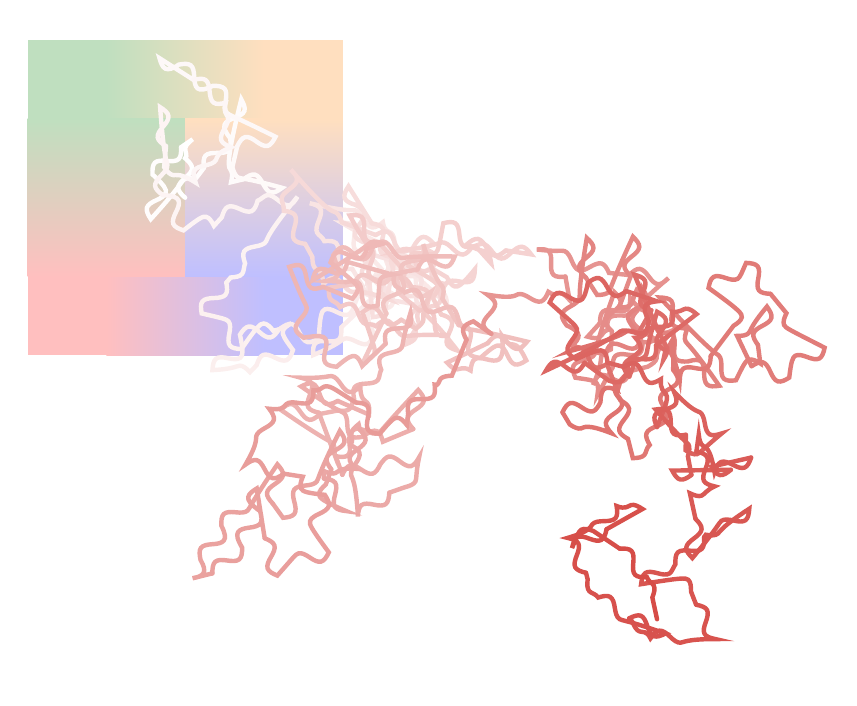
\begin{tikzpicture}[decoration={coil},dna/.style={decorate, decoration={aspect=0, segment length=0.5cm}},ultra thick,line cap=round]
  \coordinate (current) at (0,0);
  \coordinate (old) at (0,0);
  \coordinate (new) at (rand,rand);
  \foreach \i in {0,1,...,100} {
    \draw[dna,colora!\i] (current)
    .. controls ++([scale=-1]old) and
    ++(new) .. ++(rand,rand)
    coordinate (current);      
    \coordinate (old) at (new);
    \coordinate (new) at (rand,rand);
  }
  
\begin{pgfonlayer}{background}
  %\clip[xshift=-1cm] (-.5\textwidth,-.5\textheight) rectangle ++(\textwidth,\textheight);
  \colorlet{upperleft}{green!50!black!25}
  \colorlet{upperright}{orange!25}
  \colorlet{lowerleft}{red!25}
  \colorlet{lowerright}{blue!25}
     % The large rectangles:
  \fill [upperleft]  (0,0) rectangle ++(-2,2);
  \fill [upperright] (0,0) rectangle ++(2,2);
  \fill [lowerleft]  (0,0) rectangle ++(-2,-2);
  \fill [lowerright] (0,0) rectangle ++(2,-2);
    % The shadings:
  \shade [left color=upperleft,right color=upperright]
  ([xshift=-1cm]0,0) rectangle ++(2,2);
  \shade [left color=lowerleft,right color=lowerright]
      ([xshift=-1cm]0,0) rectangle ++(2,-2);
    \shade [top color=upperleft,bottom color=lowerleft]
      ([yshift=-1cm]0,0) rectangle ++(-2,2);
    \shade [top color=upperright,bottom color=lowerright]
      ([yshift=-1cm]0,0) rectangle ++(2,2);
\end{pgfonlayer}

    
\end{tikzpicture}
\end{document}
